\section{Investigation of Metrics}
\label{sect:metrics_study}
An investigation into possible metrics for determination of schedule quality.

\subsection{Introduction and rationale}
Metrics - basically quantative standards for measuring performance, quality or some aspect of a service or process we wish to monitor. In the context of scheduling these can be broadly divided into problem complexity metrics and schedule quality metrics. Problem complexity metrics (PCM) measure the difficulty of a scheduling problem and provide an independant variable with which to asses the performance of schedulers. It might be found for example that a particular scheduler which performs well on a \emph{easy} problems is out-performed by an alternative scheduler when faced with \emph{difficult} problems. Schedule quality metrics (SQM) measure the actual performance of schedulers on such problems - this in essence is what the whole project is about - the determination of the best scheduler under given conditions. A third set of metrics which will not be discussed in this section are those metrics used by the actual schedulers to perform scoring, selection, retraction and other heuristic procedures in the determination of schedules - these will be discussed in the relevant scheduler descriptions (Sect. \ref{ss:schedulers}. (XXX)

% NOTE this is a reference to one or more sections in the schedcomparch/scoringmodel etc  and future schedulers on the 
%      items used to make the thing work.

\subsection{Problem complexity metrics (PCM)}
\label{ss:pcm}
These metrics describe the complexity of the scheduling problem at any given time. In addition to there use for assessing the performance of schedulers under test, it is likely that an advanced scheduler could itself make use of these metrics by looking ahead to see where hotspots (difficult scheduling periods) are likely to occur and thus take these into account in its decision making - this would introduce a feedback effect which would make the whole exercise rather more as the degree of feedback ought to be determined and taken into account in any complexity assessment.


 The basic problem is to schedule the observations in the ODB, consequently this is where the focus of the investigation begins. The content of the observing database or pool (ODB) at any time defines the set of observations that are available for scheduling at that time. This pool evolves due to the arrival of new observing requests, modification of existing request (e.g. in light of observing results) and removal of spent requests. These modifications which may be made by observers themselves via a phase2 tool or automatically by external user agents occur in principle continuously. The complexity manifests itself through changes in the amount and severity of competition between observing requests for particular times and over the course of a night in the overall load.

These metrics will be denoted hereforth using the notation $C_x$ to indicate a \underline{c}omplexity metric with subscript, here (x) to denote a specific aspect.


\subsubsection{Contention profile $C_c$}
This is the time evolving profile of the number of observation groups which could be scheduled according to their explicit timing constraints. Additional refinements include convolving with the probability of the time actually being available based on likely weather and technical downtime forecasts. The average contention over the course of a night gives an estimate of how overloaded the schedule could potentially be. This static contention profile is a crude measure as it does not take into account the fact that some of the groups which figure in the contention profile later in the night may have already been selected by then and thus need not be considered. Another possibility is to introduce a weighted probability of execution on those groups figuring later in the night to reduce the the effect of early executions, - e.g. a simple exponential decay from $P_{avail}=1$ at the start of group's execution window with decay factor based on the group's likely execution - though how do I work that out ? - most likely this would depend on the contention statistics we are actually trying to work out ! Effects of disruptors early in the night will also change the contention later as groups which \emph{ought} to have been executed may still be in contention later. The dynamic contention profile $C_c$ is calculated by performing a forward simulation through the night and extracting actual contention in the process - this is of course somewhat dependant on the scheduler used but can be a valuable tool for assessing the degree of competition between groups

\subsubsection{Demand profile $C_d$}
A given group will potentially have multiple observing windows when it should be attempted. During any given window the group can be considered to have a demand D on the time within that window. E.g. if the group $g$ has an (estimated) execution time $X(g)$ and its window of opportunity is $\phi(g)$ \footnote[1]{this is the window during which it may legally start, it may run on over the end of the window as this is taken account of in determining whether the group could be executed} then the group's demand over that window is $D=X/(X+\phi)$. If we add up the demand contributions of all the groups which are enabled at any given time we should have a measure of how much demand is placed on that instant. If this aggregate demand exceeds unity then it is likely that some of the groups will not be observed i.e. the requirement for time is greater than the time available. 
There are several refinements that can be made on this estimate. Firstly we can work out the numerator fairly easily - it can usually be considered constant and known. The denominator is more of a problem. Firstly working out the window of opportunity from the group's time constraint window \textsf{W} is straightforward, however this window may extend from just a few minutes upto several days or even weeks. In the later case the group's target(s) may rise and set several times and the various implicit timing constraints may be broken on several occasions e.g. the lunar distance constraint will impose a varying overlap with the target visibility windows. If we consider each of the calculable constraints then we can work out the actual amount of time (within the window) that the group can
actually be observed - this gives us a revised (increased) estimate for the group's individual demand for those times within the new sub-windows. 
Going on another stage we might consider those constraints which cannot be worked out in advance. A group may have a minimum seeing constraint - we cannot tell what the seeing will be like at any future time though we may be able to estimate the likeliness of attaining the group's minimum level. Likewise we can obtain estimates of extinction (perhaps including seasonal variation). We should in addition consider the probability that the selected time is even available for observing - weather and technical downtime mean that a certain fraction of time is lost - a crude climatological estimate might just give the average probability of bad weather (averaged over long periods), we might also have more accurate seasonal-adjusted climatological information, better still if we can predict for some time ahead based on current and recently collected weather data then we shall have a better demand estimate i.e. we are calculating the likely time available rather than the certain time available for the group.

Formally:- Let $X(g)$ represent the \emph{estimated} execution time of a group $g$ and $U(g,t)$ the remaining useful time left for that group at time $t$, then the partial demand of $g$ at time $t$ is defined as:

$d(g,t) = X(g)/(X(g) + U(g,t))$ where $U(g,t) = \tau(w^*_i) \cap [t,\infty] \cap N(t) \cap M(g) \cap V(g))$ and others, where $V(g)$ is the set of visibility windows for $g$'s targets from $t$ onwards, $M(g)$ is the set of windows satisfying observing constraints, $N(t)$ the set of nights from $t$ onwards.

Some stuff on seeing/extinction stats. More on weather/technical downtime.

If a group $g$ is to execute at some future time $t$ we need to know that the weather will be good at that time and that it will remain good for at least $X(g)$. From the weather stats:- 

$P_{exec}=P_{good}(t) \dot \int_{t=X(g)}^{t=\infty}{\rho(t)dt}$ where $\rho(t)$ represents the distribution of lengths of continuous \emph{good} weather runs.

\subsubsection{Load $C_l$}
The load is a fairly simple metric which describes the ratio of executable time in a given observing night to the length of the night (or astronomical night). Simple load is calculated using the sum of execution times for each executable window of each group that can be executed during the night. It includes all windows of all groups whether they \emph{must} be executed that night or not. An urgency weighted load $C_{ul}$ can also be calculated which weights each execution time by the reciprocal of the number of remaining nights in which the window could be observed. Critical load $C_{cl}$ is a pruned version of the normal load where only groups which {\bf must} be executed that particular night are included. Priority weighted load $C_{pl}$ is calculated by taking into account all of the groups' windows which \emph{should} be executed on a given observing night (as opposed to those groups which \emph{might} be executed. The sum of execution times for each window is weighted by the priority of the group whose window it is. This is in effect the potential maximum value for the $Q_{PX}$ SQM and can be used to normalize this.

\subsection{Schedule quality metrics (SQM)}

These are the metrics used to compare the results of using different schedulers or scheduling policies on a given scheduling problem. These are needed to determine which scheduler performs best. Needless to say this is the most difficult problem for several reasons.
\begin{itemize}
\item The metric used in the selection heuristic cannot be used for the simple reason that these may be what distinguishes one scheduler from another - clearly if we use a metric $m_1$ for scheduler \emph{S\_1} and metric $m_2$ for scheduler \emph{S\_2} then measuring the performance of both schedulers using $m_1$ would naturally find that \emph{S\_1} was the better scheduler. Likewise using $m_2$ to compare the results would reveal \emph{S\_2} as the better scheduler. We therefore need a more generic metric which is ideally {\bf NOT} involved in the selection process.
\item What was that other one ?
\end{itemize}

This turns out to be particularly difficult. In the common scheduling literature there are many generic metrics used, however these all suffer from the problem that they are tuned for the generic job-shop scheduling problem in which a number of identical jobs with specified due dates have to be processed. Typical metrics include:-

\begin{itemize}
\item Slack - the amount of time where no job is in progress.
\item Tardiness - total lateness for jobs executed.
\item Throughput - total no of jobs through the system.
\item other
\end{itemize}

Can we use any of these ? The problem is that the OGs generally have a due dates which cannot be exceded - if they are late the data is of less or no use. We are not neccessarily bothered about throughput so much as the quality of the results. 

we might be able to use some of this however with suitable weighting e.g. a late high priority job is worse than a late low priority job (but by how much?). 

We can seperate out various forms of utility measure (NOTE these are discussed elsewhere but not in correct place)

User based (needs simple Phase2 specification or QOS metrics)
Enterprise based - includes scientific priorities, distribution of time between proposals.

\subsubsection{Potential utility measure} Work out the best utility that can be achieved during the night (PU) (i.e. assume we can do all the groups that could be done and do them at the best possible times) - this is after all the ultimate aim of the scheduler ! Work out the actual utility scored by the scheduler that night - the Efficiency (E) is then the ratio. May need to scale - after all if oversubscribed we could never do it all anyway try load scaling 1/L (load defined as aggregate (average) demand) or maybe better as \emph{sum of execution times of all groups that can and {\bf should} be executed tonight}. Could also try rank-scaling top(n) such that $\sum{x_i} < \tau(n)$ - I cant quite recall what I meant by that at the moment.


\subsubsection{Primitive utility measures}
There are a number of primitive measures that could be used independantly - in reality the complex tradeoffs between these make a more generic measure more useful however there is likely still some value in using these. These measures are by and large \emph{single night} measures. 

\begin{itemize}
\item Height metric $Q_H$ measures the difference between the optimum time for performing a group based on its height to transit height ratio during the night and its actual selected execution time. By adding these up we get a measure of badness - i.e. ideally all groups would get done at their highest point (in the feasibility window).

\item Optimal Height metric $Q_{OH}$ measures how close to the \emph{optimum} height the group is observed in its execution window. 

The optimum height is basically the highest elevation attained by the group during the feasible observation window - in a given window this may be at the end (rising target), start (setting target) or somewhere in the middle of the observing window (transiting target). 

There is however a non-linear relationship between elevation and airmass such that for targets which do not rise particularly high the difference in image quality between worst and best case elevation may be high over a relatively small elevation difference whereas for high rising targets the difference in airmass and hence image quality between best and worst case elevations will be small for the same elevation difference .



Consequently it may be better to measure the ratio of execution-time airmass $a_{actual}$ to best achievable airmass $a_{opt}$ as an Optimal Airmass metric $Q_{OA}$. 

Additionally, the \emph{benefit} (image quality advantage) of one airmass over another may itself be non-linear and this is what we should really be measuring. $Q_{BA}$ measures the ratio of some decreasing benefit function $b(a)$ of airmass $a$ at optimal airmass and actual execution-time airmass. A simple option for $b(a)$ would be to use the known correction  \cite{standard airmass/wavelength correction paper} of image FWHM or seeing $s$ for airmass relative to \emph{ideal} seeing at elevation $90^\circ$, $s(a)=s_{90}a^{0.6}$ with $s_{90}$ indicating the image FWHM at $z=0,a=1$ and assuming image quality is judged purely (and linearly) on FWHM. It should be noted that this correction depends also on observation wavelength $\lambda$. Figure \ref{fig:baz_plot} shows 2 models for $b(a)$ based on the standard FWHM correction.
\begin{equation}
Q_{OA} = \frac{1}{L(S)}\sum_{g \in S}{\frac{a_{opt}}{a_{actual}}}
\end{equation}
where $a = \sec{z}$ is the airmass of group's target at zenith distance $z$.

\begin{equation}
Q_{BA} = \frac{1}{L(S)}\sum_{g \in S}{\frac{b(a_{actual})}{b(a_{opt})}}
\end{equation}
where $b(a)$ represents the benefit (image quality advantage) for airmass $a$.

\item Monitor window metric $Q_{MW}$ measures the difference between the optimum time (wrt the centre of a monitor window) for performing a group based on the known monitor window and its actual selected execution time By adding these up we get a measure of badness - i.e. ideally all groups would get done at the centre of the monitor window. (there are some implications wrt non-monitor groups - how do we select the centre of the window ?. What if the window centre is not actually feasible - how is this taken into account  - do we pick nearest feasible point in window either before or after centre  - can also do something like $u(t)$ = some function which peaks at the window centre and we want the group done at t where $max_{t \in \textsf{W} \cap \textsf{T}}(U(t))$.   

\item Priority metric $Q_{PX}$ measures the total priority score achieved i.e just sums up the priorites of the groups selected weighted by the amount of time spent performing the group on the basis that e.g. an hour of high priority is better than 2 lots of 10 minutes preforming low priority groups. The final value can be normalized by dividing by the length of night (or astro-night) or perhaps better by using the priority weighted load $C_{pl}$ (see section xx) as this also gives an indication of the degree of \emph{missed opportunity}.
\begin{equation}
Q_{PX} = \frac{1}{L_N}\sum_{g \in S}{X(g,t)p(g)}
\end{equation}
where $p(g)$ is the priority value for group $g$ and $X(g,t)$ is the estimated execution time for group $g$ at execution instant $t$.

\item Target demand metric $Q_{TD}$ measures how \emph{urgent} the selected groups are with reference to the night's demand profile $C_d$.
\begin{equation}
Q_{TD} = \frac{1}{L(S)}\sum_{g \in S}{f_D(g,t)}
\end{equation}
where $f_D(g,t)$ represents the value of the demand heuristic for group $g$ at execution instant $t$.

\item Night windows count metric $Q_{NW}$ is an attempt to guage the number of nights in which a group could have been selected - it is effectively a count of the number of subwindows in which a group could be executed - a high value indicates that the scheduler is picking groups which dont have to be selected on that night, conversely a low value indicate a scheduler which is picking groups for which execution on the night is more critical. 

\item Execution target metric $Q_{XT}$ is a measure of the amount of the night during which groups are actively being observed. A low value is effectively an indication of \emph{slack time}.
\begin{equation}
Q_{XT} = \sum_{g \in S}{X(g,t)}
\end{equation}
where $X(g,t$) is the estimated execution time for group $g$ at execution instant $t$.

\item Remaining nights metric $Q_{RN}$ counts a decreasing function (for convenience 1/n) of the \emph{number of nights remaining} $n$ for any groups in the observability window $\Phi(g,t)$ at the time of selection/execution. It effectively measures how \emph{urgent} the window was in terms of the number of future chances of executing 
the group other than tonight. e.g. If a group could be executed tonight or on 3 future nights this yields a value for RN of 4 and thus 1/4 as its urgency.
\begin{equation}
Q_{RN} = \sum_{g \in S}{\frac{1}{R(g,t,\Phi(g,t))}}
\end{equation}
where $R(g,t,\phi)$ counts the number of remaining nights for a feasiblity window $\phi(g,t)$ of group $g$ at execution instant $t$ - i.e. it counts the number of feasible sub-intervals of $\Phi$ with maximum of 1 per night.

\item Yield tracking metric $Q_{YT}$ - details of this v.important.(See Appendix. \ref{sect:app_calcqy}).


\item Resource allocation/usage metrics $Q_{Ax}$ for various resources $x$ against target values. Long term only valid over period of order semester or year - TAG assigned MUF.

\item Multiple combined metrics such as $Q_{OA \cdot PX}$ would allow pairs (or larger tuples) of metrics to be combined as would linear combinations such as $w_{oa}Q_{OA}+w_{px}Q_{PX}$.

\end{itemize}
\begin{figure}[h]
\subfigure[Comparison of models for determining airmass image quality advantage ($b(z)$)]{
    \label{fig:baz_plot}
    \includegraphics[scale=0.25, angle=-90]{figures/baz_plot.eps}
  } 
\caption{Various metric models}
\end{figure}

These metrics require pre-calculation and storage prior to running the scheduler as we want to know the answer to: \emph{When is the best time to do this group on this execution for each exec of the group in the night} 


It had originally been intended to use these to minimise the sum of differences between the actual and optimal execution times - a good schedule then would be one in which the metric gave a low or best case zero result. A problem with this is that it is possible to achieve such a score by simply ommitting to perform observations - this is reminiscent of the train performance metrics used to measure the efficiency of privatized railway companies. If a train is running very late - simply cancelling the train removes it from the lateness statistics adding to the misery of the waiting passengers - its little comfort that the next train is on time if they have had to wait an hour for it !. Consequently these metrics must be scaled to give a high score when the measured variable is at maximum, lower measures when the time is poorly met and zero (or even negative) scores when the observation is not attempted. A schedule which simply avoids potential observations would then score badly. 

Note: The best schedule for a given night is the one where every {\bf critical} group is executed at its best time (ie when its overall utility is highest) and where the remaining groups (if any) are selected ``appropriately''. To determine what this actually is requires to test every feasible combination of critical group (and others) to see what could be achieved. This may then need to be done for different environmental assumptions for the night ahead. The remaining (non-critical) groups should probably be selected to miximize profit over a period (rather than for that specific night). All this makes no assumption about additional groups added via ODB mutation.


It will be useful to use ODB character metrics as an independant variable to compare E for various schedulers.

\emph{Almost any/Every} metric used for this can be used as a selection heuristic - so...


Need to look at longer term aims (i.e. those that would be introduced by a tactical/strategic planner) - these include things like- fairness between users/TAGs, distribution of environmental conditions, darkness, regularity of data product etc. It may not be neccessary however to worry about these from the scheduler's pov as it is by neccessity working on a shorter timescale - these higher order entities can force appropriate changes in the scheduler's behaviour by altering the control parameters (and metrics) used by the scheduler to satisfy their longer term aims.  
 




% This lot has also sneaked in some of it belongs in SQM section as end discussion
%
NOTE:\[This lot has also sneaked in some of it belongs in SQM section as end discussion\]
\subsubsection{Project completion}
[This has sneaked in here it belongs in the SQM advanced metrics section]
Project completion has been used as a metric for comparing scheduling policies or schedules generated by different schedulers (SPIE paper from?? and UKIRT paper). I suggest that this is not always a good metric - a project which relies on gathering data over an extended period and for which the length of data gathering, periodicity of gathering are more important would not be well served by completing the program in the fastest time. For such programs we should be more concerned with producing data at a rate which tracks the expected production rate of data. In addition we would like to generate the best quality of data or at least data of a quality which meets or exceeds the programs stated requirements - e.g. we select an observation to be done in seeing which is as good or better than required, at low airmass and any other factors which could contribute to its quality. There is a problem with this and flex-groups - they get all data in a chunk - how do we \emph{track} this?

Note: Global optimization is what we want but local optimizer may be sub-optimal e.g. of Despatch compared to (short) lookahead. Example when groups have finite and variable enablement intervals EI (use proper symbol). Should we be trying to optimize in terms of when is the best time I can do this group rather than what is the best group to do now. \emph{Description of an example with g1 long EI g2 with short EI but v.hi score. g1 selected but wipes g2's EI. Could have picked g3 with short exec then g2 - overall score is higher and still do g1 later with good score - include a diagram showing the score profiles for the groups}.




\begin{note}User preference on when to be done should be taken into account - rather than do X now just because it has highest score in a global sense, do Y because its best time to be done is now, whereas as X would prefer to be done later when its score is higher - (Granzer includes time profiles in \cite{granzer03stella})
\end{note}

\begin{note}Matching conditions to available instruments - use the instrument most suitable in present conditions - how?\end{note}

\begin{note}Useful link to Bresina's thesis chapt3 has notes on contention and demand profiles - these equate roughly to my aggregate demand profiles and tracking metric http://ic-www.arc.nasa.gov/ic/projects/xfr/sampling/thesis/index.html\end{note}


\subsubsection{Discussion on metrics/quality/reward}.
I need a way to compare the results of various schedules i.e. the result of scheduling over say a night using a given algorithm or set of parameters or despatching rule(s)/policy. What I am after is a way of measuring the cumulative reward for the night. This is not the same as a look-ahead situation where I am trying to decide what to do - this is a posterior measurment of how good a particular schedule has been.

We shall define $S(i)$ as the $i^{th}$ schedule. It contains a sequence $G(S_i) = {g_j}$ of groups, which are executed at times ${t_j}$.

There are 2 sorts of utility/reward being considered.

\begin{enumerate}
\item Enterprise utility.
The first represents the utility to the telescope, Ideally it wants to do (scientifically) valuable work and as much of it as possible. It does not want to sit about doing nothing just so it can wait for a high value observation with a small window of opportunity (graph showing a schedule snippet with 2 low value but long groups and little idle time and 2 high value (scientific priority) but short groups with a heap of idle time) if we consider the figure the low value groups give a low sum score $\sum V_i$ for the night if we just add their individual utilities whereas the high value groups give a high sum score. On the other hand if we do an integral (int V(t)) we get a better score for the low value groups. 

We may want to factor in idle time as a contribution to cumulative reward i.e. as a penalty/cost term. This can arise for several reasons:-
There may be an idle gap between groups due to the specific enablement windows, during the execution of a group we can distinguish useful and wasted time - useful time is basically exposing (and to some extend readout which we cannot avoid), wasted time includes slewing, selection and configuraton of instruments, acquisition by autoguider, settling time, and the scheduling time itself. 

Factors we might include in $V_e(g,t)$ include:-
\begin{itemize}
\item some measure of the scientific priority assigned to the group's proposal.
\item a contribution from condition matching - we dont want to waste quality time doing groups which can be executed in poorer conditions.
\end{itemize}


\item User utility.
The second approach is via a set of user-preference metrics. In the ideal schedule all the user's doable observations would be done at their optimum times. Of course we cant always work these out - we can work out when the target will be best placed e.g. at its highest elevation in the current window (bear in mind the window may extend over several nights) but we cannot say what the conditions will be like at that time - i.e. the scope may be out of action due to weather or the seeing could be horrendous. The user's preferences metric could include factors like - how close to centre of time window, how good the airmass, how well conditions are/will be matched. Each group could have a set of user-specified weights for these as they would have their own preferences as to which are more important and the relative importance of particular attribute values. One user might prefer his observations to be done at low airmass rather than worrying too much about timeliness, another might want his timing adhered to rigidly and not care so much about the airmass - the group's observing constraints define limits for these attributes.

Factors we might include in $V_u(g,t)$ include:-
\begin{itemize}
\item airmass preference
\item sky brightness
\item seeing matching
\item window position
\item data profile tracking
\end{itemize}

\end{enumerate}

We can also work out the utility $u_i(t)$ for a group over the night, this will have some maximum value $u^*_i(t)$ in any given night - this is the optimum time to do the group so we could work out $u_i(t)/u^*_i(t)$ so the utilities are normalized - do we need to do that?

Maybe we want something like.
\begin{equation}
V(S_i) = \mathop{\sum}_{g_j \in G(S_i)} ((w_{u}*V_{u}(g_j,t_j) + w_{e}*V_{e}(g_j,t_j))*\tau_j - c_j u_j) 
\end{equation} 
where $u_j$ is the amount of useless/unproductive time in the $j^{th}$ group execution, $w_{u}$ is the weighting for user-pref satisfaction, $V_{u}(g_j)$ is the value the user assigns to the performing of his observation at the selected time, $w_{e}$ is the weighting for enterprise value, $V_{e}(g_j)$ is the value of scientific priority assigned to the chosen observations, $\tau_j$ is the useful time part of the group's execution - (we are integrating, or are we ?)

This metric adds in the contribution from enterprise and user-preference matching but since all users are free to specify their own weightings does this cause any problems with comparison? e.g. If user-A assigns preferences so his observations are always good i.e. he has no preference and user-B chooses his preferences so his observations are best at t\_B, user-A will get a better score contribution most of the time - this may not matter - we are not using this to select A over B just to measure the selection score over the night?


\subsubsection{Efficiency measure - $E$}
Given a utility measure $F(g,t)$ which describes the value of performing group $g$ at time $t$, the potential utility metric is the sum of the individual values of $F(g,t^*)$ for each group execution window on the night ${n}$ containing $t$ at the time $t^*$ which maximizes  $F(g,t)$ for that group. In other words it is the total utility which could be achieved that night if all feasible groups were executed at their optimum time. In reality it may not actually be possible to achieve this as several groups could be optimal at the same time or overlapping times. Also if the total execution time potential for the night exceeds the available night-time hours it ill not be possible even without overlaps. The metric can of course be scaled by a factor $\tau({n})/\sum_{g \in G{(n)}}{X(g)}$. The perrormance metric then becomes $E_{{S}}/E_{potential}$  where $E_{{S}} = \sum_{g \in {S}(g)}{F(g,t^*)} $. 


\subsubsection{More about contention to squeeze into discussion above}
There is a need to measure the contention for time among the groups enabled on a nightly basis, it would be useful to be able to do this on a fine granularity - e.g. minute by minute. First we must decide what we mean by contention. My definition is the degree of demand by all enabled groups for a given slice of time - put simply, if a group needs 10 minutes to execute and there is a 30 minute window of opportunity in which it can start, then its demand for the whole of this window is 10/30. If there are other groups which also have some demand for all or part of the window then they will contribute appropriate amounts to the total demand for the window to those fractions of the window during which they are enabled, the total (aggregate) demand at a given time then is the sum of all the partial demands from each group whose enablement interval includes that time. Put more formally:

$T(t) = \sum_{g : w \cap t} { \frac{t_x(g)}{w_e(g)} }$ 

TODO this needs writing properly 
TODO also need some formal definitions for w/W/tx etc and where they are got from.

How then do we calculate this ? The numerator is the easiest - define the components of this along with any uncertainty terms and consideration of parallelism - this is obtained from the ExecModel. First we must decide what we mean by enablement window. Each group has by reason of its TimingConstraint a set of one or more windows in which it is intended to observe (execute) the group (also called a visit in some systems - need a distinct word), in the case of a Flex group this is a single window [ts,te]. For a periodic monitoring group there will be a series of windows $w_i = [ts+i*p-w/2, ts+i*p+w/2]$ such that the last window stops around $t_e$. As a first approximation then the denominator can just be considered to be the size of any window which includes t - (Note no group should by definition of the various timing constraint classes have more than one window corresponding to any given time). Because we have an optical telescope and observe only at night, we can restrict the actual time available to a group for the execution of its observing window to the intersection of the window with the night which includes t. So $t_avail = W \cap N(t)$, thus incresasing the contention contribution. A number of additional approximations will continue to pare this denominator down so we can expect the first approximation to be significantly low. We should note some points here. I have so far assumed implicitly that the group's window of opportunity W is less than the duration of a single night, this will often not be the case, i.e. many group windows extend over serveral days (and nights) and in some case, especially long activation flexible groups may run for weeks or months, so the actual $t_avail$ in these cases should really be represented by W intersect {N} where N is the set of all the future nights for which the group is available. We cannot stop here, just because it is night does not mean we can make the observation, the target will not neccessarily be visible, either above the geographical horizon or any operational horizon of the telescope, so we can further reduce the available time by considering only the part of the night(s) where the target(s) are visible $t_avail = W \cap N \cap V$. Each group has associated with it a number of observing constraints - some of these represent implicit additional time constraints, namely those which can be calculated in advance. An example would be the lunar distance constraint - the observations in the group cannot be made if the moon is less than some given distance from the observation's target. If we add these into the mix we get an extra reduction in the available time for the group to execute - bearing in mind that these calculations must be performed for all future nights which intersect the group's window containing t. We have done all that is possible with the certain knowledge of the observing environment, there remain however a number of uncertainties - we have not considered either those observing constraints which refer to environmental conditions which cannot be predicted in advance with any certainty, e.g. the group's available window will most likely be reduced further if the seeing is worse than the maximum specified in the seeing constraint, similar things may be said concerning other unpredictable elements. (which). We can further reduce the available window if we can predict when the telescope will be unable to observe due to poor weather, mechanical or technical faults, engineering and other downtime. If we can at least obtain some statistical values for these, which may contain seasonal or other variations (e.g. weather downtime, or seeing distribution dependant on time of year) or we can predict sky and weather conditions for the night ahead with some accuracy (this will help for short period monitors) then we can get produce weighted contention profiles.


\begin{note}This is just some discussion about utility measures...should be elsewhere
What is the goal of the SE? A definition of the S+P process is \emph{to maximize the profit of the enterprise} \cite{miyashita96distributed}. This sums it up quite well. The enterprise is the telescope or the group which runs it. Profit refers here to some reward the \emph{owners} expect to get from providing the facility. This could be money - in terms of grants recieved for the continued provision and expansion of the service and could refer to some general sort of kudos within the scientific community resulting from the perception of the current and potential users that it is a novel and useful world class facility. To this end the we need to be able to measure a quantifiable reward resulting from performing the most scientifically useful or \emph{in-vogue} research. We need some way for the scheduler to select observations which will generate the highest cumulative reward and on a consistent basis, i.e. we need metrics to classify groups of potentially schedulable groups over time. 

Proposals have already been vetted and prioritized by the allocation committees so this provides a useful metric. The individual users will have some preferrences on when and under what conditions their observations are performed. They are able to specify the minimum conditions and the timing intervals and various constraints on their observations but these preferences are not ordered in any way - e.g. one user might prefer that their observations are done at low airmass and be less concerned with regularity whilst another user may be less concerned with airmass but more so with regularity - the simple constraints do not allow these preferences to be taken into account, instead a generic preference weighting is applied by the scheduler so that all observations are treated as if the users had the same preference weighting. 

The scheduler is basically answering the question - \emph{What is the best thing I can do now from those things available ?} rather than the possibly more useful from the users' pov \emph{When are the best times these available observation could be done ?}. If we can allow the user's own preference weighting to be taken into account then we will have a more user-centred view of the schedule. How can we do this? There are several options.

We can always consider the scheduling process to be a competition between users (groups of observations) for particular time slots. After the scheduling process is completed by whatever means it represents the best allocation of times to groups. In reality we do not expect to be able to extract a full schedule to cover say a whole night due to the dynamically changing environment, however we do still want to get the best observations at each time slot whether by selecting individual groups at the time (despatching) or small selections of groups over a short horizon during which the conditions (and goals) are predicted to remain reasonably stable. 

An obvious direction to follow is the auction path. We could allow the users, in reality some per-proposal delegate (agent) acting on the user's behalf to bid for time available slots as they became available. One would image the SE deciding the current time horizon based on environmental stability predictions, perhaps predicting goal evolution (P2DB evolution) on the basis of past behaviour and using knowledge of RCS future commitments (e.g. RTI or calibration time), then advertising the time slot(s) available to interested delegates. The delegates would examine their groups' requirements and decide whether to bid for any slots. More advanced (and $O^n$ more difficult) - combinatorial auctions.
\end{note}
